%%%%%%%%%%%%%%%%%%%%%%%%%%%%%%%%%%%%%%%%%%%%%%%%%%%%%%%%%%%%%%%%
\fe{\section{Procédures utilisateur}}{\section{User procedures}}
\label{util_proc}
%%%%%%%%%%%%%%%%%%%%%%%%%%%%%%%%%%%%%%%%%%%%%%%%%%%%%%%%%%%%%%%%

\begin{frame}{\fe{Procédures utilisateur}{User procedures}}{\fe{Mode d'emploi}{Instructions for use}}
  \begin{itemize}
    \item[] \fe{Il existe 7 appels à des procédures utilisateurs\\ à différentes étapes de l'algorithme de \kwo{PASAPAS}}
               {There are 7 calls to user procedures\\ at different steps of \kwo{PASAPAS} algorithm}
    \begin{center}
      \kwv{PERSO1~~PERSO2~~REEV\_MEC~~REEV\_THE}\\
      \kwv{CHARMECA~~CHARTHER~~PARATHER}
    \end{center}
  \end{itemize}
  \begin{enumerate}
    \item \fe{\g{\blue{Choisir la procédure}}\\
              selon son emplacement dans \kwo{PASAPAS} et l'action désirée}
             {\g{\blue{Choose the procedure}}\\
              according to its location in \kwo{PASAPAS} and the action required}\\
    \scriptsize
    \fe{\ding{43}\emph{par exemple : puisque \kwv{PERSO1} est appelée après le calcul d’un pas de temps,\\
        ~~~elle peut servir à modifier le suivant (conditions aux limites, matériau \dots)}}
       {\ding{43}\emph{for instance: since \kwv{PERSO1} is called after computing a time step,\\
        ~~~it can be used to update the next one (boundary conditions, material \dots)}}
    \normalsize
    \item \fe{\g{\blue{Observer la syntaxe de la procédure}}\\
              dans le code de \kwv{PASAPAS} \dots~ou bien voir le tableau suivant}
             {\g{\blue{Analyze the procedure syntax}}\\
              in the \kwv{PASAPAS} code \dots~or see table on next slide}
  \end{enumerate}
\end{frame}

\begin{frame}{\fe{Procédures utilisateur}{User procedures}}{\fe{Mode d'emploi}{Instructions for use}}
  \begin{enumerate}\addtocounter{enumi}{2}
    \item \fe{\g{\blue{Définir la procédure}}
              \lstinputlisting[language=gibiane, firstline=29, lastline=31]{dgibi/exemples.dgibi}}
             {\g{\blue{Define the procedure}}
              \lstinputlisting[language=gibiane, firstline=32, lastline=34]{dgibi/exemples.dgibi}}
    \item \fe{\g{\blue{Brancher la procédure dans}} \kwo{PASAPAS}}
             {\g{\blue{Plug the procedure in}} \kwo{PASAPAS}}
          \lstinputlisting[language=gibiane, firstline=36, lastline=42]{dgibi/exemples.dgibi}
  \end{enumerate}
\end{frame}

\begin{frame}{\fe{Procédures utilisateur}{User procedures}}{\fe{Liste des procédures}{List of procedures}}
%  \begin{spacing}{1}
  \tiny
  \fe{\begin{tabular}{lllp{3cm}}
        \g{Procédure}             & \g{Indice dans la table PASAPAS}           & \g{Syntaxe}                                 & \g{Rôle possible} \\
        \hline\\
        \kwv{PERSO1}              & \kwg{'PROCEDURE\_PERSO1'~~}\kw{ = VRAI ;}  & \kwv{PERSO1 }\kw{tab1 ;}                    & Mise à jour du problème après calcul du pas mécanique\\
                                  &                                            &                                             & \\
        \kwv{REEV\_MEC}           & \kwg{'PROCEDURE\_REEV\_MEC'}\kw{ = VRAI ;} & \kwv{REEV\_MEC }\kw{tab1 n1 ;}              & Idem, mais dans la \red{boucle thermo mécanique}\\
                                  &                                            &                                             & \\
        \kwv{CHARMECA}            & \kwg{'PROCEDURE\_CHARMECA'}\kw{ = VRAI ;}  & \kw{tab2 = }\kwv{CHARMECA}\kw{ tab1 tps1 ;} & Ajout chargements mécaniques pendant \kwo{UNPAS}\\
                                  &                                            &                                             & \\
        \kwv{PERSO2}              & \kwg{'PROCEDURE\_PERSO2'~~}\kw{ = VRAI ;}  & \kwv{PERSO2 }\kw{tab1 ;}                    & Mise à jour du problème après calcul du pas thermique\\
                                  &                                            &                                             & \\
        \kwv{REEV\_THE}           & \kwg{'PROCEDURE\_REEV\_THE'}\kw{ = VRAI ;} & \kwv{REEV\_THE }\kw{tab1 n1 ;}              & Idem, mais dans la \red{boucle thermo mécanique}\\
                                  &                                            &                                             & \\
        \kwv{CHARTHER}            & \kwg{'PROCEDURE\_CHARTHER'}\kw{ = VRAI ;}  & \kw{tab2 = }\kwv{CHARTHER}\kw{ tab1 tps1 ;} & Ajout chargements thermiques pendant \kwo{TRANSNON}\\
                                  &                                            &                                             & \\
        \kwv{PARATHER}            & \kwg{'PROCEDURE\_PARATHER'}\kw{ = VRAI ;}  & \kwv{PARATHER}\kw{ tab1 tps1 ;}             & Mise à jour variables externes des caractéristiques thermiques\\
      \end{tabular}}
     {\begin{tabular}{lllp{3.2cm}}
        \g{Procedure}             & \g{Index in PASAPAS table}                 & \g{Syntax}                                  & \g{Possible function} \\
        \hline\\
        \kwv{PERSO1}              & \kwg{'PROCEDURE\_PERSO1'~~}\kw{ = VRAI ;}  & \kwv{PERSO1 }\kw{tab1 ;}                    & Updates the problem after the mechanical calculation step\\
                                  &                                            &                                             & \\
        \kwv{REEV\_MEC}           & \kwg{'PROCEDURE\_REEV\_MEC'}\kw{ = VRAI ;} & \kwv{REEV\_MEC }\kw{tab1 n1 ;}              & Ditto, but in the \red{thermo mechanical loop}\\
                                  &                                            &                                             & \\
        \kwv{CHARMECA}            & \kwg{'PROCEDURE\_CHARMECA'}\kw{ = VRAI ;}  & \kw{tab2 = }\kwv{CHARMECA}\kw{ tab1 tps1 ;} & Mechanical loads addition during \kwo{UNPAS} iterations\\
                                  &                                            &                                             & \\
        \kwv{PERSO2}              & \kwg{'PROCEDURE\_PERSO2'~~}\kw{ = VRAI ;}  & \kwv{PERSO2 }\kw{tab1 ;}                    & Updates the problem after the thermal calculation step\\
                                  &                                            &                                             & \\
        \kwv{REEV\_THE}           & \kwg{'PROCEDURE\_REEV\_THE'}\kw{ = VRAI ;} & \kwv{REEV\_THE }\kw{tab1 n1 ;}              & Ditto, but in the \red{thermo mechanical loop}\\
                                  &                                            &                                             & \\
        \kwv{CHARTHER}            & \kwg{'PROCEDURE\_CHARTHER'}\kw{ = VRAI ;}  & \kw{tab2 = }\kwv{CHARTHER}\kw{ tab1 tps1 ;} & Thermal loads addition during \kwo{TRANSNON} iterations\\
                                  &                                            &                                             & \\
        \kwv{PARATHER}            & \kwg{'PROCEDURE\_PARATHER'}\kw{ = VRAI ;}  & \kwv{PARATHER}\kw{ tab1 tps1 ;}             & Updating of the external variables of thermal parameters\\
      \end{tabular}}
  \fe{Avec :}{With:}
  \begin{tabular}{llll}
    \kw{t1} & \fe{: la table de \kwo{PASAPAS}}{: the \kwo{PASAPAS} table}                                    & \kw{tps1} & \fe{: l’instant de calcul courant}{: the current calulated time}\\
    \kw{n1} & \fe{: le numéro d'appel de la procédure (0 ou 1)}{: the call number of the procedure (0 or 1)} & \kw{t2}   & \fe{: la table de sortie (pour \kwv{CHARMECA} et \kwv{CHARTHER})}{: the output table (for \kwv{CHARMECA} et \kwv{CHARTHER})}
  \end{tabular}
  \normalsize
%  \end{spacing}
\end{frame}

\begin{frame}{\fe{Procédures utilisateur}{User procedures}}{\fe{Quelques remarques}{A few remarks}}
  \small
  \begin{itemize}
    \item \fe{Les instructions dans ces procédures sont libres !}{Instructions inside these procedures are free!}
    \item \fe{\kwo{CHARMECA} et \kwo{CHARTHER} doivent sortir une table, avec 2 indices possibles :}
             {\kwo{CHARMECA} and \kwo{CHARTHER} output is a table with 2 possible indexes:}
      \begin{tabular}{lp{7cm}}
        \kwg{'ADDI\_MATRICE'} & \fe{qui contient les matrices de RIGIDITE que l'on veut ajouter au 1er membre}
                                   {contains the stiffness matrices (RIGIDITE type object) to be added to the 1st member}\\
        \kwg{'ADDI\_SECOND'}  & \fe{qui contient les CHPOINT que l'on veut ajouter au 2nd membre (forces nodales, \dots)}
                                   {contains the CHPOINT to be added to the 2nd member (nodal forces, \dots)}
      \end{tabular}
    \item \fe{En grands déplacements (option \kwg{'GRANDS\_DEPLACEMENTS'})\\ \kwo{CHARMECA} est appelée sur la configuration déformée}
             {For large displacements (\kwg{'GRANDS\_DEPLACEMENTS'} option)\\ \kwo{CHARMECA} is called on the deformed shape}
  \end{itemize}
\end{frame}

\begin{frame}{\fe{Procédures utilisateur}{User procedures}}
             {\fe{Exemple : éprouvette entaillée en traction}
                 {Example: notched specimen under traction}}
  \footnotesize
  \begin{itemize}
    \begin{textblock*}{6cm}(8.5cm,0cm)
      \begin{tikzpicture}
        \node[anchor=south west,inner sep=0] (image) at (0,0)
        {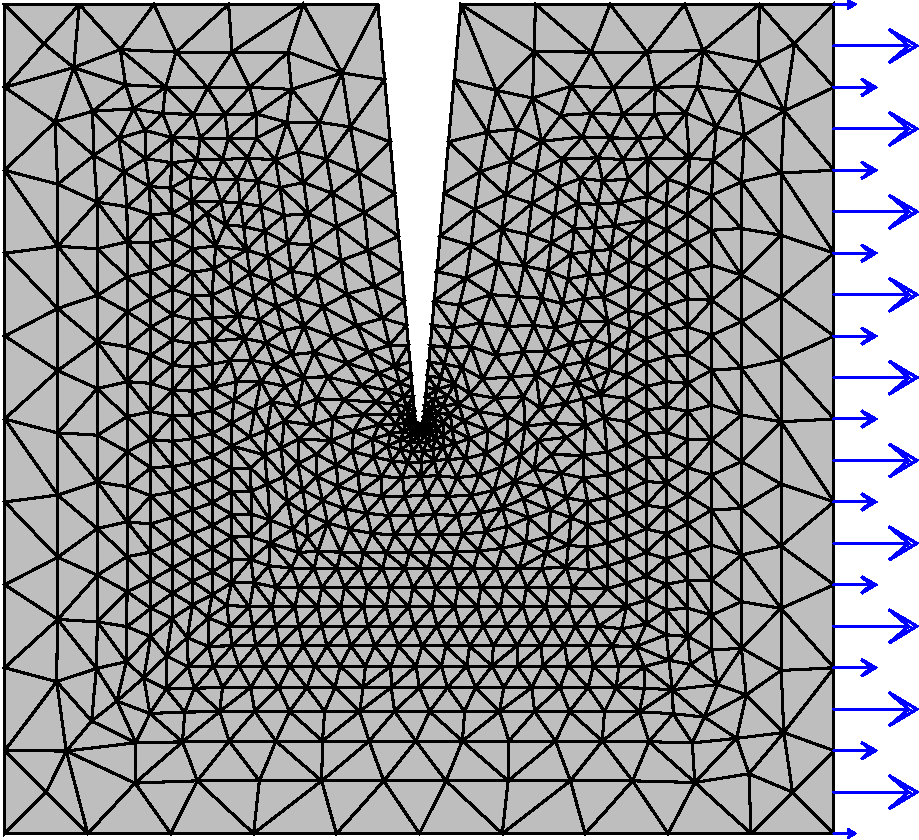
\includegraphics[width=3cm]{images/exemple/exemple_0.1}};
        \begin{scope}[x={(image.south east)},y={(image.north west)},color=black]
          \draw (0.37,1.04) node {\tiny \kw{p7}};
          \draw (0.55,1.04) node {\tiny \kw{p4}};
        \end{scope}
      \end{tikzpicture}
    \end{textblock*}
    \lstinputlisting[basicstyle=\ttfamily\tiny, language=gibiane, firstline=7, lastline=30]{dgibi/exemple_perso1.dgibi}
    \item[]
  \end{itemize}
\end{frame}

\begin{frame}{\fe{Procédures utilisateur}{User procedures}}
             {\fe{Exemple : éprouvette entaillée en traction}
                 {Example: notched specimen under traction}}
  \footnotesize
  \begin{itemize}
    \begin{textblock*}{6cm}(8.5cm,0.33cm)
      \begin{tikzpicture}
        \node[anchor=south west,inner sep=0] (image) at (0,0)
        {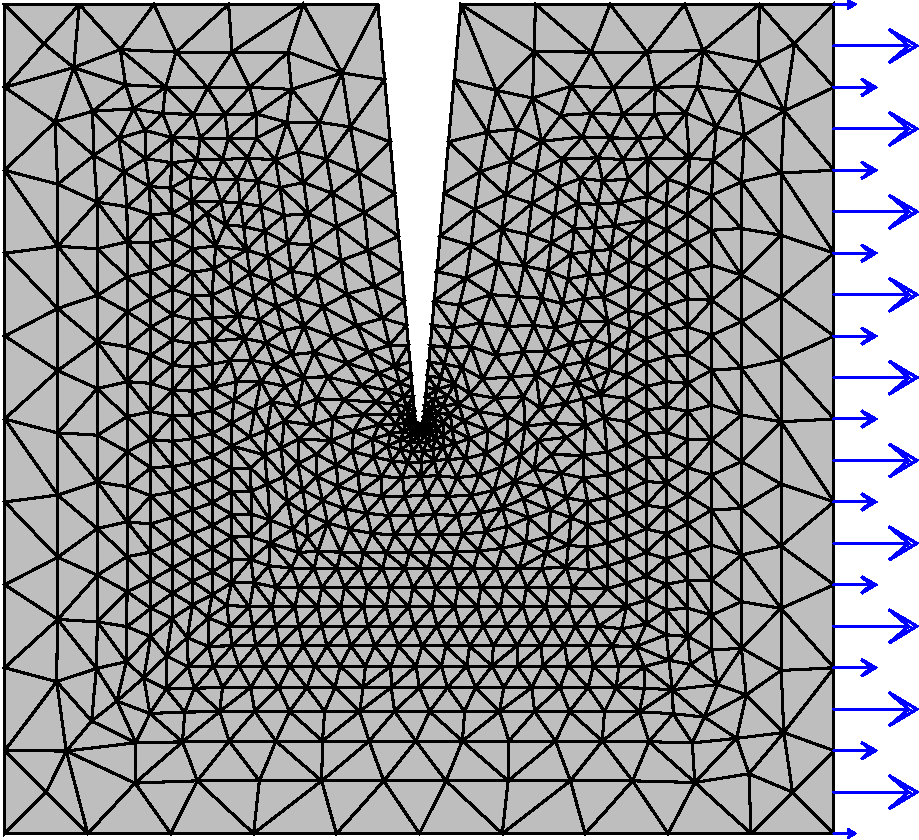
\includegraphics[width=3cm]{images/exemple/exemple_0.1}};
        \begin{scope}[x={(image.south east)},y={(image.north west)},color=black]
          \draw (0.37,1.04) node {\tiny \kw{p7}};
          \draw (0.55,1.04) node {\tiny \kw{p4}};
        \end{scope}
      \end{tikzpicture}
    \end{textblock*}
    \begin{textblock*}{6cm}(8.5cm,3.5cm)
      \animategraphics[controls,loop,poster=last,width=3.6cm]{10}{images/exemple/exemple_1.}{01}{21}
    \end{textblock*}
    \lstinputlisting[basicstyle=\ttfamily\tiny, language=gibiane, firstline=32, lastline=61]{dgibi/exemple_perso1.dgibi}
    \item[]
  \end{itemize}
\end{frame}

\begin{frame}{\fe{Procédures utilisateur}{User procedures}}
             {\fe{Exemple : éprouvette entaillée en traction \red{+ flexion pilotée par l'ouverture}}
                 {Example: notched specimen under traction \red{+ bending controled by opening}}}
  \footnotesize
  \begin{itemize}
    \begin{textblock*}{6cm}(8.5cm,0.33cm)
      \begin{tikzpicture}
        \node[anchor=south west,inner sep=0] (image) at (0,0)
        {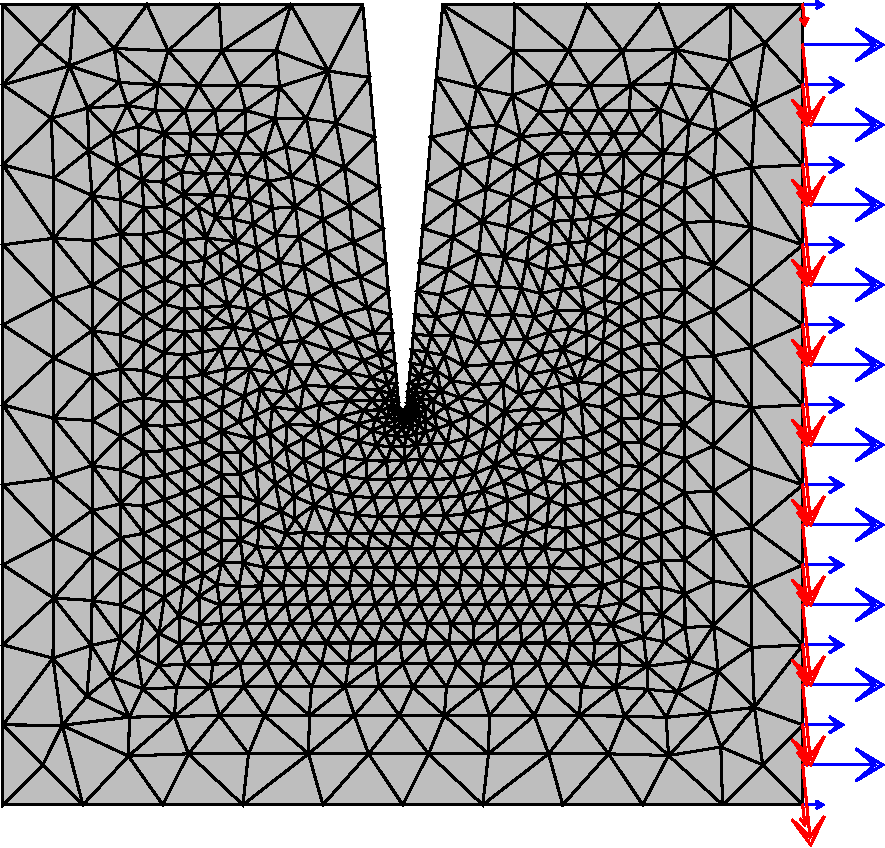
\includegraphics[width=3cm]{images/exemple/exemple_0.2}};
        \begin{scope}[x={(image.south east)},y={(image.north west)},color=black]
          \draw (0.37,1.04) node {\tiny \kw{p7}};
          \draw (0.55,1.04) node {\tiny \kw{p4}};
          \draw[<->, red] (0.41,1.) -- (0.5,1.);
          \draw (0.5,0.9) node[anchor=west, fill=white] {\tiny $\red{\Delta u}$};
        \end{scope}
      \end{tikzpicture}
    \end{textblock*}
    \begin{textblock*}{6cm}(8.5cm,3.5cm)
      \animategraphics[controls,loop,poster=last,width=3.6cm]{10}{images/exemple/exemple_2.}{01}{21}
    \end{textblock*}
    \lstinputlisting[basicstyle=\ttfamily\tiny, language=gibiane, firstline=68, lastline=97]{dgibi/exemple_perso1.dgibi}
    \item[]
  \end{itemize}
\end{frame}
